\section{Methodology}
\label{sec:methodology}
This section introduces \emph{\ours}, a physics-guided approach for removing lens flare in event cameras. We derive a \textbf{forward model} of flare formation, whose exact inversion is intractable (Sec.~\ref{ssec:forward_model}), motivating a learning-based solution. Building on this, we develop a two-stage strategy: a \textbf{physics-driven simulator} for large-scale paired training data (Sec.~\ref{ssec:simulator}) and a \textbf{real-world acquisition system} for robust validation (Sec.~\ref{ssec:real_data_acquisition}). We then define the learning objective and restoration network. The overview framework is illustrated in Fig.~\ref{fig:methodology-flowchart}.


\begin{figure*}[!t]
    \centering
    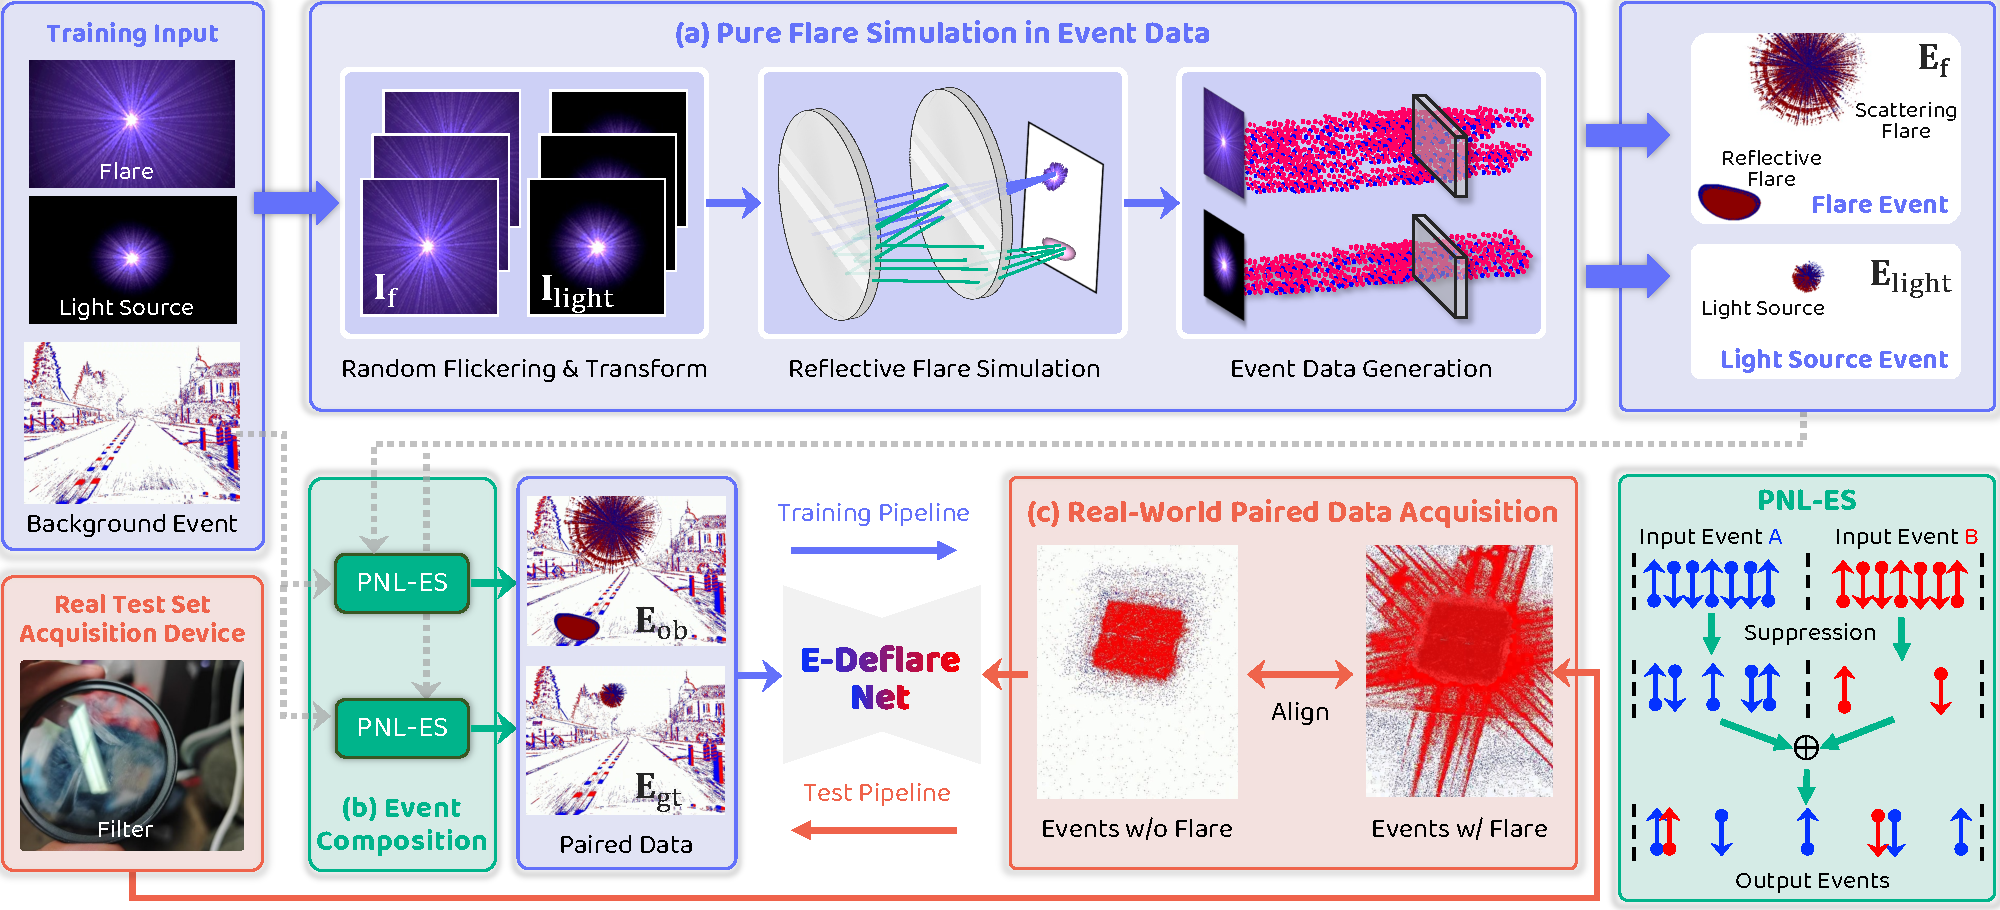
\includegraphics[width=\textwidth]{figures/pipeline.pdf}
    \vspace{-0.5cm}
    \caption{\textbf{Data Generation, Training \& Validation.} 
    In the \emph{\ours}~framework, we introduce two parallel pipelines to address data scarcity. 
    The training pipeline synthesizes paired data by first generating dynamic flare events from static images (\eg, Flare7K++) and then fusing them with real background events (\eg, DSEC) via our physics-guided PNL-ES operator. 
    The testing pipeline captures paired real-world data using a controllable optical setup. A removable filter allows us to record the same dynamic scene \emph{w/} and \emph{w/o} flare, which forms our validation set after post-processing.
    }
    \vspace{-0.2cm}
    \label{fig:methodology-flowchart}
\end{figure*}



\subsection{Physical Modeling of Flare in Events}
\label{ssec:forward_model}

To model lens flare in event streams, we establish a physical model of the \emph{scene} and \emph{imaging process}, decomposing the total irradiance into background $\mathbf{I}_{\mathrm{bg}}$ and a primary light source $\mathbf{I}_{\mathrm{light}}$. Under an \textbf{ideal lens} $\mathcal{L}_{\mathrm{ideal}}$, both components are perfectly imaged, producing the clean, flare-free ground-truth irradiance:
\begin{equation}
    \mathbf{I}_{\mathrm{gt}}(x, y, t) = \mathbf{I}_{\mathrm{bg}}(x, y, t) + \mathbf{I}_{\mathrm{light}}(x, y, t)~.
\end{equation}
In contrast, a \textbf{real lens} $\mathcal{L}_{\mathrm{real}}$ introduces reflections and scattering that corrupt this formation. While the background remains largely unaffected, the bright light source produces a spatially expansive, structured flare component $\mathbf{I}_{\textcolor{ev_red}{\mathrm{\mathbf{f}}}}$ that subsumes both the distorted direct illumination and the additional scattered energy, thereby replacing $\mathbf{I}_{\mathrm{light}}$ in the observed irradiance. The observed irradiance $\mathbf{I}_{\mathrm{ob}}$ can thus be approximated by a linear superposition in the intensity domain~\cite{dai2022flare7k,wu2021train,dai2024flare7k++}. This process is formulated as follows:
\begin{equation}
    \mathbf{I}_{\mathrm{ob}}(x, y, t) \approx \mathbf{I}_{\mathrm{bg}}(x, y, t) + \mathbf{I}_{\textcolor{ev_red}{\mathrm{\mathbf{f}}}}(x, y, t)~.
\label{eq:image_superposition_final}
\end{equation}
This intensity-domain corruption occurs \emph{before} the sensor and forms the foundation of our event-level analysis. For brevity, we omit coordinates $(x, y)$ where context is clear.

An event camera sensor $\mathcal{S}_{\mathrm{evt}}(\cdot)$ operates on this corrupted irradiance $\mathbf{I}_{\mathrm{ob}}$. Unlike conventional cameras that capture frames at fixed intervals, $\mathcal{S}_{\mathrm{evt}}$ is a stateful process: each pixel independently monitors its log-intensity $L(t) = \log(\mathbf{I}_{\mathrm{ob}}(t))$ and asynchronously triggers an event when the accumulated change exceeds a contrast threshold $c$. Mathematically, an event is fired at time $t_i$ when:
\begin{equation}
    |L(t_i) - L(t_{\mathrm{last}})| \ge c~,
    \label{eq:event_threshold_condition}
\end{equation}
where $t_{\mathrm{last}}$ denotes the timestamp of the preceding event at that pixel. The polarity $p_i = \mathrm{sign}(L(t_i) - L(t_{\mathrm{last}})) \in \{+1, -1\}$ encodes the direction of the intensity change. The resulting event stream $\mathbf{E}(t)$ can be represented as:
\begin{equation}
    \mathbf{E}(t) = \mathcal{S}_{\mathrm{evt}}(\mathbf{I}_{\mathrm{ob}}(t)) = \sum\nolimits_{i} p_i \delta(t - t_i)~,
    \label{eq:event_stream_definition}
\end{equation}
where $\delta(\cdot)$ is the Dirac delta function. This yields an integral relationship between log-intensity and $\mathbf{E}(t)$:
\begin{equation}
    L(t) = c \int_{0}^{t} \mathbf{E}(\tau) \, d\tau + L(0) + \varepsilon(t)~,
    \label{eq:sensor_model_integral_redef}
\end{equation}
where $L(0)$ is the initial log-intensity and $\varepsilon(t)$ represents the \emph{total intensity residual}. This term aggregates all signal components not encoded in the event stream. It mainly comprises two parts: \textbf{(1)} the \textbf{sub-threshold quantization error}, which is bounded by the threshold $c$, and \textbf{(2)} \textbf{sensor noise} (\eg, shot noise, threshold variance), which is stochastic and may accumulate over time. While modern sensors strive to minimize noise, $\varepsilon(t)$ remains an intrinsic and unavoidable part of the underlying physical process.

\textbf{Dual Mathematical Representation.} To establish the physical interaction mechanism between background and flare events, we first recognize that the event stream $\mathbf{E}(t)$, though discrete, admits a continuous interpretation through its temporal derivative relationship. Differentiating Eq.~\ref{eq:sensor_model_integral_redef}, the rate of change of log-intensity can be expressed as:
\begin{equation}
    \frac{dL(t)}{dt} = c \cdot \mathbf{E}(t) + \xi(t)~,
    \label{eq:continuous_link}
\end{equation}
where $\xi(t) \triangleq d\varepsilon(t)/dt$ is the \emph{residual rate}. Eq.~\ref{eq:continuous_link} bridges the discrete and continuous domains.


\textbf{Log-Derivative Mixing.} The linear superposition of irradiance (Eq.~\ref{eq:image_superposition_final}) becomes highly non-linear when mapped to the logarithmic domain. Differentiating $L_{\mathrm{ob}}(t) = \log(\mathbf{I}_{\mathrm{bg}}(t) + \mathbf{I}_{\textcolor{ev_red}{\mathrm{\mathbf{f}}}}(t))$ via the chain rule gives:
\begin{equation}
    \frac{dL_{\mathrm{ob}}(t)}{dt} = w_{\mathrm{bg}}(t) \frac{dL_{\mathrm{bg}}(t)}{dt} + w_{\textcolor{ev_red}{\mathrm{\mathbf{f}}}}(t) \frac{dL_{\textcolor{ev_red}{\mathrm{\mathbf{f}}}}(t)}{dt}~,
    \label{eq:log_derivative_mixing}
\end{equation}
where $L_{\mathrm{bg}}(t) \triangleq \log \mathbf{I}_{\mathrm{bg}}(t)$ and $L_{\textcolor{ev_red}{\mathrm{\mathbf{f}}}}(t) \triangleq \log \mathbf{I}_{\textcolor{ev_red}{\mathrm{\mathbf{f}}}}(t)$, and the coefficients are defined as:
\begin{equation}
    w_{\mathrm{bg}}(t) = \frac{\mathbf{I}_{\mathrm{bg}}(t)}{\mathbf{I}_{\mathrm{bg}}(t) + \mathbf{I}_{\textcolor{ev_red}{\mathrm{\mathbf{f}}}}(t)}~,~~ w_{\textcolor{ev_red}{\mathrm{\mathbf{f}}}}(t) = 1-w_{\mathrm{bg}}(t)~.
    \label{eq:weights_definition}
\end{equation}
This reveals that although intensities superpose linearly, their logarithmic derivatives mix through a weighted sum: the physical origin of the \textbf{non-linear suppression effect}.


\textbf{Complete Forward Model.} Substituting the dual representation (\ie, Eq.~\ref{eq:continuous_link}) into Eq.~\ref{eq:log_derivative_mixing}, we obtain:
\begin{equation}
    \begin{aligned}
    \frac{dL_{\mathrm{ob}}(t)}{dt} ={}&
    w_{\mathrm{bg}}(t) \left[ c \mathbf{E}_{\mathrm{bg}}(t) + \xi_{\mathrm{bg}}(t) \right] \\
    &+ w_{\textcolor{ev_red}{\mathrm{\mathbf{f}}}}(t)
    \left[ c \mathbf{E}_{\textcolor{ev_red}{\mathrm{\mathbf{f}}}}(t)
    + \xi_{\textcolor{ev_red}{\mathrm{\mathbf{f}}}}(t) \right]~,
    \end{aligned}
    \label{eq:full_mixing_derivative}
\end{equation}
where $\xi_{\mathrm{bg}}(t)$ and $\xi_{\textcolor{ev_red}{\mathrm{\mathbf{f}}}}(t)$ denote the respective residual rates. Integrating Eq.~\ref{eq:full_mixing_derivative} over time and substituting back into the sensor model (Eq.~\ref{eq:sensor_model_integral_redef}) yields the complete forward model:
\begin{equation}
    \mathbf{E}_{\mathrm{ob}}(t) = \mathcal{S}_{\mathrm{evt}}\left( \exp\left( \int_{0}^{t} \Phi(\tau) \, d\tau + L_{\mathrm{ob}}(0) \right) \right)~,
    \label{eq:full_forward_model}
\end{equation}
where the integrand $\Phi(\tau)$ represents:
\begin{equation}
    \begin{aligned}
    \Phi(\tau) ={}&
    w_{\mathrm{bg}}(\tau)\, c \mathbf{E}_{\mathrm{bg}}(\tau)
    + w_{\textcolor{ev_red}{\mathrm{\mathbf{f}}}}(\tau)\, c \mathbf{E}_{\textcolor{ev_red}{\mathrm{\mathbf{f}}}}(\tau) \\
    &+ w_{\mathrm{bg}}(\tau)\,\xi_{\mathrm{bg}}(\tau)
    + w_{\textcolor{ev_red}{\mathrm{\mathbf{f}}}}(\tau)\,\xi_{\textcolor{ev_red}{\mathrm{\mathbf{f}}}}(\tau)~.
    \end{aligned}
    \label{eq:integrand_phi}
\end{equation}
The first line contains the weighted impulse terms, and the second line contains the mixed residuals $\xi_{\mathrm{mix}}$. This formulation is physically complete: the outer operator $\mathcal{S}_{\mathrm{evt}}$ ensures the output is a discrete event stream (Eq.~\ref{eq:event_stream_definition}), while the integral captures the accumulated log-intensity change, explaining why flare-dominated regions exhibit slower accumulation, and thus suppressed background events.


\textbf{Practical Considerations.} If continuous irradiance profiles $\mathbf{I}_{\mathrm{bg}}(t)$ and $\mathbf{I}_{\textcolor{ev_red}{\mathrm{\mathbf{f}}}}(t)$ were known, one could compute $w(t)$ and $\xi_{\mathrm{mix}}$ and evaluate $\mathcal{S}_{\mathrm{evt}}$ exactly. In practice, however, complete and accurate irradiance information is unavailable, so $\mathbf{I}(t)$, the weights, and the residual terms cannot be recovered. Exact integration is therefore intractable, motivating the discrete approximation in Sec.~\ref{ssec:simulator}.



\subsection{Physics-Driven Simulator for Paired Data}
\label{ssec:simulator}


As illustrated in Fig.~\ref{fig:methodology-flowchart}, the pipeline operates in two stages: \textbf{Stage 1} generates pure flare events by extending image-based methods~\cite{dai2024flare7k++} to the event domain, while \textbf{Stage 2 implements the physics-driven event composition mechanism}, the core contribution of this work.


$\bullet$~\textbf{Stage 1: Pure Flare Simulation in Events.}
The first stage synthesizes pure event streams for the light source under a non-ideal lens ($\mathbf{E}_{\textcolor{ev_red}{\mathrm{\mathbf{f}}}}$) and an ideal lens ($\mathbf{E}_{\mathrm{light}}$). Real paired dynamic captures would be ideal but are scarce; even image-domain paired flare videos are rare. We therefore use Flare7K++ \cite{dai2024flare7k++}, the only training-scale paired source, and animate its static assets.

To address this, we decompose the flare into two components. For the \textbf{scattering flare}, whose pattern varies smoothly with the light source's position, we generate dynamic videos by applying complex temporal effects to the static Flare7K++ assets. These include random spatial transformations and intensity flickering. For the \textbf{reflective flare}, whose intricate patterns change drastically and cannot be realistically interpolated from static images, we use a dedicated \textbf{Reflective Flare Simulation} module to synthesize its dynamic intensity video. The final video sums both components. These are processed by a standard event simulator~\cite{lin2022dvs} to produce $\mathbf{E}_{\textcolor{ev_red}{\mathrm{\mathbf{f}}}}$ and $\mathbf{E}_{\mathrm{light}}$.


$\bullet$~\textbf{Stage 2: Physics-Driven Event Composition.}
As established in Sec.~\ref{ssec:forward_model}, exactly evaluating the forward model requires continuous irradiance $\mathbf{I}(t)$, which is unavailable during synthesis. A naive heuristic is to directly merge the two streams ($\mathbf{E}_{\mathrm{ob}} \approx \mathbf{E}_{\mathrm{bg}} \cup \mathbf{E}_{\textcolor{ev_red}{\mathrm{\mathbf{f}}}}$), which implicitly assumes $w_{\mathrm{bg}} = w_{\textcolor{ev_red}{\mathrm{\mathbf{f}}}} = 1$ and ignores the normalized weighting entirely. This is physically incorrect: in the extreme case where flare irradiance dominates ($\mathbf{I}_{\textcolor{ev_red}{\mathrm{\mathbf{f}}}} \gg \mathbf{I}_{\mathrm{bg}}$), the physical weight $w_{\mathrm{bg}} \to 0$ and background events should be almost entirely suppressed. Direct addition erroneously preserves all of them, producing training data that fundamentally misrepresents the sensor response.

To implement the physical weighting under this constraint, we introduce the \emph{Probabilistic Non-Linear Event Suppression} (\textbf{PNL-ES}) operator $\oplus$. PNL-ES independently retains each background event with probability $w_{\mathrm{bg}}(t)$ and each flare event with probability $w_{\textcolor{ev_red}{\mathrm{\mathbf{f}}}}(t)$, then combines the survivors into a single stream; this is fundamentally different from direct union, which implicitly sets both probabilities to one and discards the weighting. The physical justification follows from Eq.~\ref{eq:full_mixing_derivative}: each background impulse advances $L_{\mathrm{ob}}$ by only $w_{\mathrm{bg}}(t)\cdot c$ rather than the full threshold $c$, so the expected fraction of background events surviving to trigger an observed event is exactly $w_{\mathrm{bg}}(t)$. As a concrete example, when $\mathbf{I}_{\textcolor{ev_red}{\mathrm{\mathbf{f}}}} \gg \mathbf{I}_{\mathrm{bg}}$ (a common scenario near bright light sources), $w_{\mathrm{bg}} \to 0$ and background events should be nearly eliminated; direct union would erroneously preserve all of them. Since continuous $\mathbf{I}(t)$ is unavailable, we estimate the weights from intensity proxies; because PNL-ES is probabilistic, inexact estimates do not yield a single incorrect simulation but instead produce varied training samples spanning a realistic distribution of suppression states, providing principled physics-guided augmentation rather than a deterministic reconstruction.

Using this operator, we construct both the flare-corrupted input and its corresponding clean ground truth, that is:
\begin{equation}
    \mathbf{E}_{\mathrm{ob}} = \mathbf{E}_{\mathrm{bg}} \oplus \mathbf{E}_{\textcolor{ev_red}{\mathrm{\mathbf{f}}}} , \quad
\mathbf{E}_{\mathrm{gt}} = \mathbf{E}_{\mathrm{bg}} \oplus \mathbf{E}_{\mathrm{light}}~.
\end{equation}
The required data assets are assembled accordingly. Real-world background events $\mathbf{E}_{\mathrm{bg}}$ with diverse real-world motion are sampled from DSEC~\cite{gehrig2021dsec}, while intensity profiles for retention probability are obtained from Stage 1's synthetic outputs ($\mathbf{I}_{\textcolor{ev_red}{\mathrm{\mathbf{f}}}}$ and $\mathbf{I}_{\mathrm{light}}$) and estimated from the available event data ($\mathbf{I}_{\mathrm{bg}}$), all of which are sufficient for the probabilistic PNL-ES formulation.


This pipeline yields a large-scale, physically grounded training dataset. By anchoring synthesis to real background events (which dominate event density), we mitigate the sim-to-real gap of fully synthetic systems. As validated below, this facilitates generalization to \emph{real-world} data.



\subsection{Real-World Paired Data Acquisition}
\label{ssec:real_data_acquisition}

Validation faces the practical impossibility of capturing \emph{perfectly aligned} scene pairs with and without flare. Inspired by image-based strategies~\cite{dai2022flare7k, dai2024flare7k++}, we adapt this general capture strategy to event cameras.

\textbf{Capture Setup.} We mount a removable optical filter (\eg, six-line star filters) in front of the lens (Fig.~\ref{fig:methodology-flowchart}). The protocol involves two consecutive recordings of the same scene: one with the filter in place to capture the flare-corrupted stream $\mathbf{E}_{\mathrm{ob}}$, and another immediately after its removal to acquire the near-clean reference $\tilde{\mathbf{E}}_{\mathrm{gt}}$. Multiple filter types introduce diversity in flare patterns.

\textbf{Event-Specific Alignment Strategy.} Unlike frame-based cameras, event cameras possess microsecond-level temporal sensitivity, making precise alignment difficult if either the camera or the scene moves; this is why no such paired dataset currently exists. To address this, we fix the camera and illuminate with high-frequency flickering light sources (\eg, LED arrays). Spatial alignment follows automatically; temporal alignment is achieved by synchronizing streams to the flickering pattern. This yields a small-scale but high-fidelity real-world validation set.

\begin{figure}[!t]
    \centering
    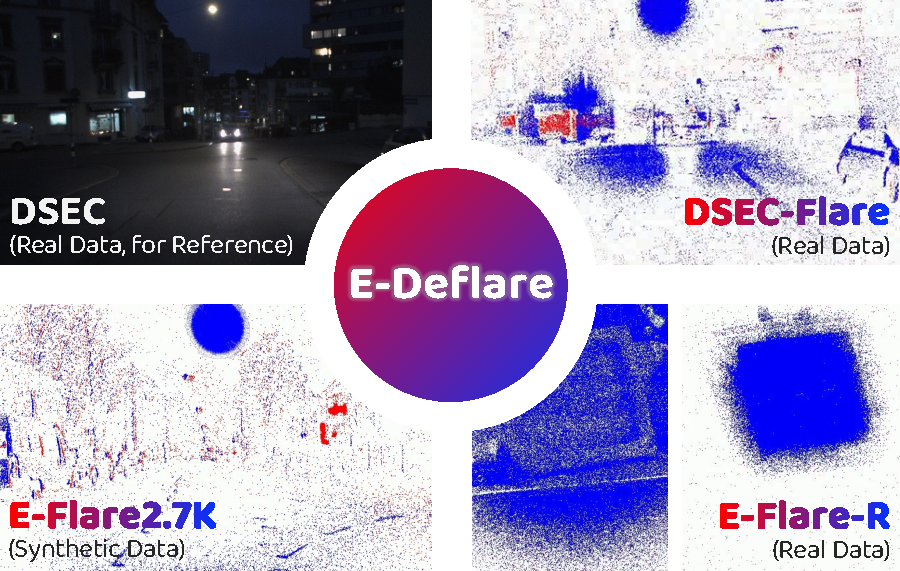
\includegraphics[width=\columnwidth]{figures/2x2.pdf}
    \vspace{-0.65cm}
    \caption{Data samples from our benchmark, shown alongside a reference RGB frame (top left). The benchmark includes: a real-world flare example from \textbf{DSEC-Flare} (top right); a synthetic sample from \textbf{E-Flare2.7K} (bottom left); and a paired real-world sample from our test set \textbf{E-Flare-R} (bottom right).}
    \label{fig:2x2}
\end{figure}
\textbf{Post-Processing.} The captured stream $\tilde{\mathbf{E}}_{\mathrm{gt}}$ undergoes residual artifact suppression (facilitated by the known light source geometry) and metric-guided spatio-temporal refinement to yield the final ground truth $\mathbf{E}_{\mathrm{gt}}$. While this protocol is designed for controlled validation and does not cover scenarios involving camera or scene motion, we complement it with DSEC-Flare, a large-scale collection of unpaired real-world flare examples mined from public datasets. Though lacking ground-truth alignment, DSEC-Flare provides diverse and challenging flare patterns that allow qualitative assessment of generalization beyond controlled settings, thus serving as a complementary benchmark to our paired test set.


We then train E-DeflareNet to validate our data pipeline and theoretical analysis. Event streams are converted to voxel grids $\mathcal{V}(\cdot)$~\cite{duan2021eventzoom}. Using a standard 3D U-Net~\cite{cciccek20163d} with residual prediction, we optimize:
\begin{equation}
\theta^* = \underset{\theta}{\arg\min} \left\| \mathcal{V}(\mathbf{E}_{\mathrm{ob}}) + f_{\theta}(\mathcal{V}(\mathbf{E}_{\mathrm{ob}})) - \mathcal{V}(\mathbf{E}_{\mathrm{gt}}) \right\|_2^2.
\end{equation}
The restored voxel grid is $\hat{\mathcal{V}}_{\mathrm{gt}} = \mathcal{V}(\mathbf{E}_{\mathrm{ob}}) + f_{\theta}(\mathcal{V}(\mathbf{E}_{\mathrm{ob}}))$. 
% Details are in the \textbf{Appendix}.


\subsection{Datasets \& Benchmark}
The \emph{\ours}~benchmark comprises three complementary datasets, each serving a distinct role:
\begin{itemize}
    \item \textbf{\underline{E-Flare2.7K}:} A large-scale \emph{simulated} dataset for training and quantitative testing, with $2.7$K samples ($2{,}545$ training, $175$ testing). Light-source positions and flare patterns are randomized; see the \textbf{Appendix} for examples.

    \item \textbf{\underline{E-Flare-R}:} A paired \emph{real-world} test set for high-fidelity validation under controlled acquisition, providing $150$ samples with optical artifacts such as surface glare and internal reflections~\cite{shi2023identifying}.

    \item \textbf{\underline{DSEC-Flare}:} Curated sequences from the public DSEC dataset~\cite{gehrig2021dsec} exhibiting natural flare corruption in driving scenarios, used for qualitative real-world evaluation where paired ground truth is not needed.
\end{itemize}

\iffalse
\begin{table}[!t]
    \centering
    \small
    \caption{Overview of the proposed datasets in \emph{\ours}~benchmark.}
    \vspace{0.1cm}
    \label{tab:dataset_overview}
    \begin{tabular}{lccc}
    \toprule
    \textbf{Dataset} & \textbf{Type} & \textbf{Paired} & \textbf{Bkg.} \\
    \midrule
    E-Flare2.7K & Synth. & \checkmark & \checkmark \\
    E-Flare-R   & Real   & \checkmark & --         \\
    DSEC-Flare  & Real   & --         & \checkmark \\
    \bottomrule
    \end{tabular}
    \vspace{-0.2cm}
\end{table}
\fi
Together, these datasets cover large-scale learning, paired real-world evaluation, and qualitative evidence in natural driving scenes, which cannot be obtained from a single acquisition source. Some representative data samples are in \cref{fig:2x2}. Further details are provided in the \textbf{Appendix}.
